\documentclass[a4paper,11pt]{article}

%%%%%%%%%%%%%%%%%%%%%%%%%%%%%%%%%%%%%%%%%%%%%%%%%%%%%%%%%%%%%%%%%%%%%%
%%% packages (and their customizations)
%%%%%%%%%%%%%%%%%%%%%%%%%%%%%%%%%%%%%%%%%%%%%%%%%%%%%%%%%%%%%%%%%%%%%%
\usepackage[utf8]{inputenc}
\usepackage{hyperref}
\usepackage{authblk}
\usepackage{amsmath}
\usepackage{amsthm}
\usepackage{amsfonts}
\usepackage[margin=2cm]{geometry}
\usepackage[tt=false]{libertine}
\usepackage{xifthen}
\usepackage[x11names,rgb]{xcolor}
\usepackage{fixme}
\fxsetup{status=draft, theme=color, layout={inline}}
\renewcommand{\fixmelogo}{\textcolor{black}{\colorbox{Firebrick1}%
    {\textsf{\textbf{FIX}}}}}
\usepackage{url}
\urlstyle{same}                 % same font as in text
\usepackage{booktabs}
\usepackage{setspace}
\usepackage{tikz}
\usepackage{mathtools}
\mathtoolsset{showonlyrefs}

\newcommand{\tk}{\tilde{k}}
\newcommand{\hc}{\hat{c}}
\newcommand{\figwidth}{\linewidth}

% bibliography
\usepackage[style=authoryear]{biblatex}
\addbibresource{/home/tamas/research/bibliography/references.bib}
%\addbibresource{./bibliography.bib}

%%%%%%%%%%%%%%%%%%%%%%%%%%%%%%%%%%%%%%%%%%%%%%%%%%%%%%%%%%%%%%%%%%%%%%
%%% general macros
%%%%%%%%%%%%%%%%%%%%%%%%%%%%%%%%%%%%%%%%%%%%%%%%%%%%%%%%%%%%%%%%%%%%%%

\begin{document}

\title{Consistent future approximation in continuous time}
\author{Tam\'as K.~Papp\thanks{\url{tkpapp@gmail.com}}}
\date{\today}
\maketitle

\begin{abstract}
  Analysis of the ``consistent future approximation'' method of \textcite{den2015exact} applied for a simple continuous time model: the deterministic Ramsey model. I show that while the method is easy to set up, solving the nonlinear system requires nontrivial methods for even a simple system, and once solved, the resulting residuals of the Euler equation are large compared to collocation methods, but still small enough in absolute magitude to make the model useful in practice, especially for making an initial guess about functional forms in collocations methods. 
\end{abstract}

\begin{center}
  \textsl{See the repository at \url{https://github.com/tpapp/exact-present} 
    for the accompanying code in \textsc{Julia}\nocite{bezanson17:_julia}.}
\end{center}

\paragraph{Introduction.}

Continuous time models have been used extensively in macroeconomics, finance, and other fields\footnote{References are too numerous to list here. See \textcite{acemoglu2008introduction} for a textbook based almost entirely on continuous time models, \textcite{dixit1996investment} for applications to inverstment. Applications in portfolio choice and finance started with \textcite{merton1971optimum}.} However, while in finance it is common practice to solve continuous models numerically (see \textcite{hull2009options} for commonly used methods), in macroeconomics practical applications of numerical methods usually focus on discrete time problems, despite the fact that commonly used textbooks on numerical methods address continuous-time methods.\footnote{Eg \textcite{judd98:_numer_method_in_econom} and \textcite{miranda02:_applied_comput_econom_and_finan}. Recent exceptions include \textcite{kaplan2016monetary} and related papers.}

While one of the reasons for this may be unfamiliarity with continuous-time building blocks such as Itô and Lévy processes,\footnote{For an introduction, see \textcite{oksendal2005applied}.} the other difficulty is finding a solution to the resulting functional equations. When using projection methods, functional forms that describe optimal choices and values are approximated using function families with finitely many parameters. Since in continuous time there is no general contraction mapping equivalent to value iteration in discrete time, usually the only option is to solve these problems using general nonlinear solvers, which are not guaranteed to converge, especially when the starting point is not close enough to the solution.\footnote{\textcite{kushner2013numerical} presents an alternative method, using discrete-time approximations of continuous processes.}

\textcite{den2015exact} propose a method for finding approximate solutions to discrete time systems described by a functional equation, by approximating policy functions with a linear (or similarly simple) form and imposing consistency between present and future policies around a particular state. In this short note I show that this method can be applied to continuous time systems, and examine its practicality and accuracy in the context of one of the simplest continuous time models, the deterministic Ramsey model. The advantage of this model is that it is relatively well-studied,\footnote{\textcite{aruoba2006comparing} compare a variety of numerical methods for the discrete-time version of this model with a stochastic productivity.} and it is sufficient for making the following points about the proposed method in continuous time:
\begin{enumerate}
\item The method is fast, but the resulting nonlinear system may have multiple roots even in a simple setting, so that it must be solved with care, preferably from a good initial guess. In this note I used continuation methods, starting from around the steady state.
\item The method is not very accurate when compared to collocation methods: Euler equation residuals deteriorate very quickly with distance form the steady state. For example, at half the steady state capital, the relative residual was $10^{-2}$, while a simple collocation methods $10^{-4}$ Chebyshev polynomials can easily achieve $10^{-4}$. However, it is still more than accurate enough as a starting point, so it can be used as an initial guess about the functional form for collocation methods.
\item The method is good at capturing the general shape of the policy function even near singularities, where collocation methods usually break down without transformations.
\end{enumerate}

\paragraph{Setup.} Consider a deterministic Ramsey model in continuous time, with CRRA utility function (IES $\theta$), discount rate $\rho$, production function
\begin{equation}
  F(k) = A k^\alpha - \delta k
\end{equation}
and capital accumulation equation
\begin{equation}
  \label{eq:capital-accumulation}
  \dot{k}_t = F(k_t) - c_t
\end{equation}
The most frequently used form of the Euler equation, usually obtained from the Hamiltonian, is\footnote{Eg see \textcite[Chapter 8]{acemoglu2008introduction}.}
\begin{equation}
  \label{eq:Euler-equation-t}
  \frac{\dot{c}_t}{c_t} = \frac{1}{\theta} \bigl( F'(k_t) - \rho \bigr)
\end{equation}
First, I rewrite this into a recursive form. We are solving for the policy function $c(k)$, and thus
\begin{equation}
  \dot{c} = c'(k) \dot{k} = c'(k) \bigl( F(k) - c(k) \bigr)
\end{equation}
where I have used \eqref{eq:capital-accumulation} and dropped time indices. Plugging into~\eqref{eq:Euler-equation-t}, we obtain
\begin{equation}
  \label{eq:Euler-elasticity}
  \frac{c'(k)}{c(k)} \bigl( F(k) - c(k) \bigr) = \frac{1}{\theta} \bigl(F'(k)-\rho\bigr)
\end{equation}
We cast this into the form
\begin{equation}
  \label{eq:Euler-equation}
  c'(k) \bigl( F(k) - c(k) \bigr) = \frac{1}{\theta} \bigl(F'(k)-\rho\bigr) c(k)
\end{equation}
which should be easier to manipulate. We are looking for the solution $c(k)$ to \eqref{eq:Euler-equation}.

\paragraph{Methodology.} The key to the method outlined in \textcite{den2015exact} is the following:
\begin{enumerate}
\item fix $k$,
\item assume a functional form for $c(k)$ around this point,
\item solve \eqref{eq:Euler-equation} by imposing that this form holds ``locally'', as described below.
\end{enumerate}
For simplicity, we choose a linear form
\begin{equation}
  \label{eq:linear-c}
  c(\tk; k) = c_0(k) + c_1(k)(\tk-k)
\end{equation}
First, from \eqref{eq:Euler-equation} and \eqref{eq:linear-c} we obtain
\begin{equation}
  \label{eq:linear-Euler}
  c_1(k)\bigl( F(k) - c_0(k) \bigr) = \frac{1}{\theta}\bigl( F'(k) - \rho \bigr) c_0(k)
\end{equation}
Implicit differentiation by $k$ yields
\begin{equation}
  \label{eq:implicit}
  c'_1(k)\bigl( F(k) - c_0(k) \bigr) + c_1(k)\bigl( F'(k) - c'_0(k) \bigr) =
  \frac{1}{\theta}\biggl[ F''(k) c_0(k) + \bigl( F'(k) - \rho \bigr) c'_0(k) \biggr]
\end{equation}
The method makes two assumptions. First, we impose that the approximation is \emph{valid locally} around $k$:
\begin{equation}
  \label{eq:local-validity}
  c'_0(k) = c_1(k)
\end{equation}
This would hold if the $c(\tk;k)$ was tangent to the approximated policy function $c_0(k)$. Also, we impose that for a small change in $k$, there is \emph{no first-order change in the approximating slope} $c_1(k)$:
\begin{equation}
  \label{eq:no-change-in-slope}
  c'_1(k) = 0
\end{equation}
\emph{This is a crucial assumption}, as it basically imposes no curvature. The accuracy of the method will be determined by how realistic these assumptions are. Using~\eqref{eq:local-validity} and \eqref{eq:no-change-in-slope}, \eqref{eq:implicit} becomes
\begin{equation}
  \label{eq:implicit-simple}
  c_1(k)\bigl( F'(k) - c_1(k) \bigr) = \frac{1}{\theta}\biggl[ F''(k) c_0(k) + \bigl( F'(k) - \rho \bigr) c_1(k) \biggr]
\end{equation}
For each $k$, we solve the system of \eqref{eq:linear-c} and \eqref{eq:implicit-simple}.
Note that \eqref{eq:implicit-simple} still takes the curvature of $F$ into account.

\paragraph{Numerical methods.}

Note that the system \eqref{eq:linear-Euler} and \eqref{eq:implicit-simple} is quadratic. Using random starting points and quasi-Newton methods,\footnote{Unless stated otherwise, in this note I use quasi-Newton methods with automatic differentiation \parencite{RevelsLubinPapamarkou2016}.} I generally found  \emph{three} solutions: the ``right'' one ($c_1(k), c_0(k) > 0$), a trivial one $c_1(k) = c_0(k) = 0$, and an an economically nonsensical one (with $c_1(k) < 0$). Consequently, reformulating the problem and using initial guesses is beneficial. Using \eqref{eq:Euler-elasticity} rules out the zero solution. Also note that since the steady state capital can be obtained as
\begin{equation}
  k_s = \left(\frac{\delta+\rho}{A\alpha}\right)^{1/(\alpha-1)}
\end{equation}
and $c_s=c_0(k) = F(k_s)$, an exact solution can be easily obtained at the steady state. However, even with seemingly sensible initial guesses (eg consumption and its derivative proportional to the steady state), I frequently ran into the nonsensical root, so I used the following simple continuation method:
\begin{enumerate}
\item for a $k$ near $k_s$, use initial guesses $c_0(k)=c_s$, and $c_1(k)$ from \eqref{eq:implicit-simple},
\item for other $k$, find a nearby $\tk$ for which we have solved the problem, and use $c_0(\tk), c_1(\tk)$.
\end{enumerate}

\paragraph{Solution and discussion.}

I solve on the range $k \in (0.2 k_s, 2 k_s)$, with parameters $A=1$, $\alpha=0.3$, $\rho=0.02$, $\delta=0.05$, $\theta=2$. For comparison, I solve \eqref{eq:Euler-elasticity} using a collocation method with 10 Chebyshev polynomials, which is very accurate and will be useful for comparison. I refer to the latter as the ``exact'' solution $\hc(k)$, since the approximation error has no practical relevance. This solution is referred to in the graphs as ``collocation'', while the method of \textcite{den2015exact} is labeled as ``consistent future''.

Figure~\ref{fig:ck} shows the policy function. The deviation from the exact solution is small but visible, with the exact solution method overpredicting consumption both above and below the steady state. More importantly, as can be seen in Figure~\ref{fig:ckprime} which shows the same comparison for $c_1(k)$ and and $\hc'(k)$, with the consistent future method overpredicting $c'(k)$ above and underpredicting it below the steady state, respectively. Also, note that \eqref{eq:no-change-in-slope} is violated since $c_1(k)$ appears to have significant curvature.

Figure~\ref{fig:cderiv-consistentfuture} checks \eqref{eq:local-validity} by plotting $c_1(0)$ and $c_0'(k)$, calculating the latter from a local quadratic curve. While \eqref{eq:local-validity} holds at the steady state by construction, it is violated significantly the further we move from the steady state: as $k$ approaches $0$, $c_0'(k) \approx 2 c_1(k)$. If we are aiming for a globally accurate solution, \eqref{eq:local-validity} turns out to be an unreasonable assumption. Figure~\ref{fig:policy-tangents} shows $c_0(k)$, but with tangents drawn using $c_0(k)$ and $c_1(k)$. This is another graphical illustration of the volation of \eqref{eq:local-validity}.

Figures~\ref{fig:euler-residual-consistentfuture} and \ref{fig:eulerresid-collocation} show the residual of \eqref{eq:Euler-elasticity} for the consistent future and collocation methods, respectively. Graphing this residual is a standard procedure of evaluating collocation methods \parencite{boyd2001chebyshev, judd98:_numer_method_in_econom}, since the residual can be considered as a unitless prediction error. Note that because of the errors discussed above, the consistent future method displays relatively low accuracy when compared to collocation methods, however, the residual is still small for practical purposes.

One remarkable feature of the consistent future method is that because of its locality, it does not break down as $k\to0$, In contrast to collocation methods, which require transformations or more gridpoints in areas of high curvature. This again makes it ideal for initial guesses and exploratory analysis.

\paragraph{Conclusion.} I examined the accuracy of the method proposed by \textcite{den2015exact} in the context of a simple continuous time Ramsey model, and found that it is much less accurate than collocation methods. Note, however, that the method is still reasonably accurate, and since it can be implemented very easily, it may be a good first pass approach to study the solution of functional equations. In particular, it can be used for exploratory analysis, or to provide initial guesses for nonlinear solvers in collocation methods, and since it can be evaluated at any points, it can also be used to check the assumptions about functional forms that underlie more complex methods, such as sparse grid approximations \parencite{judd2014smolyak}. The only part which requires more care is solving the nonlinear system. With these in mind, the method may be a useful addition to our toolkit for solving functional equations in economics.

\printbibliography

\begin{figure}[b]
  \centering
  \begin{minipage}[t]{0.48\linewidth}
    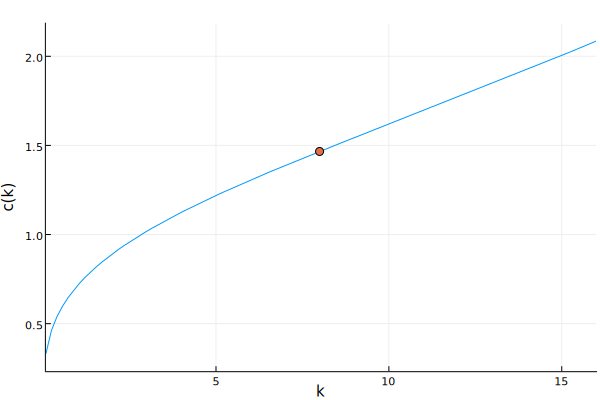
\includegraphics[width=\figwidth]{../fig/ck.pdf}
    \caption{Policy functions (consistent future: dashed, collocation: solid, steady state: dot).}
    \label{fig:ck}
  \end{minipage}\hfill%
  \begin{minipage}[t]{0.48\linewidth}
    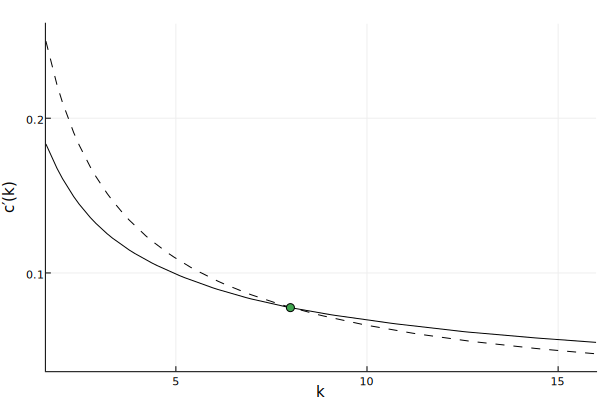
\includegraphics[width=\figwidth]{../fig/ckprime.pdf}
    \caption{$c_1(k)$ for consistent future approximation (dashed), $c'(k)$ for collocation (solid), steady state (dot).}
    \label{fig:ckprime}
  \end{minipage}
  \begin{minipage}[t]{0.48\linewidth}
    \includegraphics[width=\figwidth]{../fig/cderiv-consistentfuture.pdf}
    \caption{$c_1(k)$ (solid) and $\partial c_0(k)/ \partial k$ (dashed), the latter calculated from a local quadratic approximation.}
    \label{fig:cderiv-consistentfuture}
  \end{minipage}\hfill%
  \begin{minipage}[t]{0.48\linewidth}
    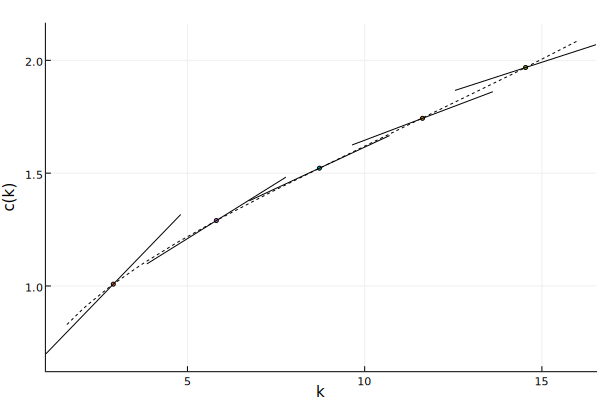
\includegraphics[width=\figwidth]{../fig/ck-tangents-consistentfuture.pdf}
    \caption{Policy function $c_0(k)$, with tangents drawn according to $c_1(k)$.}
    \label{fig:policy-tangents}
  \end{minipage}
  \begin{minipage}[t]{0.48\linewidth}
    \includegraphics[width=\figwidth]{../fig/eulerresid-consistentfuture.pdf}
    \caption{Residual of equation \eqref{eq:Euler-elasticity} for the consistent future method.}
    \label{fig:euler-residual-consistentfuture}
  \end{minipage}\hfill%
  \begin{minipage}[t]{0.48\linewidth}
    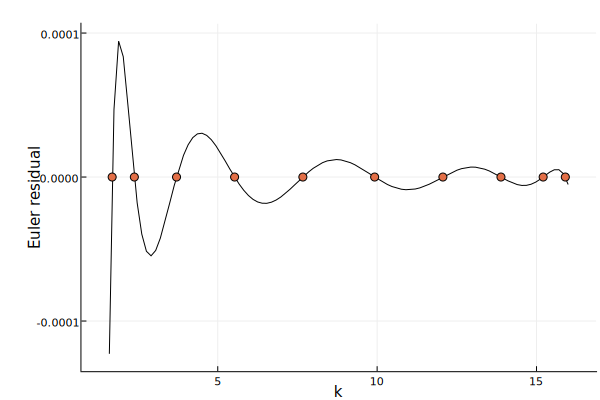
\includegraphics[width=\figwidth]{../fig/eulerresid-collocation.pdf}
    \caption{Residual of equation \eqref{eq:Euler-elasticity} for the collocation method, with collocation nodes.}
    \label{fig:eulerresid-collocation}
  \end{minipage}
\end{figure}

\end{document}
